\problemname{Triangelskolan}

Kajsa går i Triangelskolan, vars profil är att lägga runda plastbrickor så de bildar liksidiga
trianglar. Två exempel visas i figuren. Givet hur många brickor Kajsa har, skriv ett program
som beräknar sidlängden för den största triangeln hon kan skapa.
\begin{figure}[ht!]
\centering
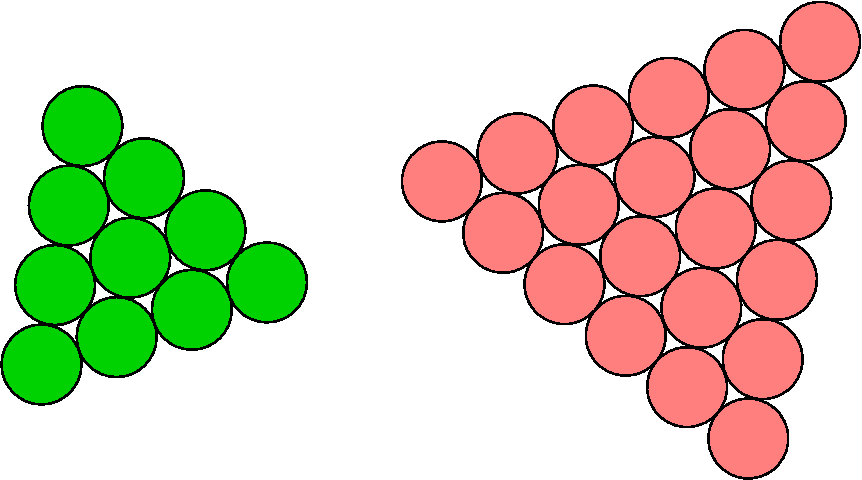
\includegraphics[width=7cm]{triangel.png}
\caption{}
\label{fig1}
\end{figure}

\section*{Indata}
Indata består av heltalet $N$ ($1 \leq N \leq 10^6$), antalet brickor Kajsa har.

\section*{Utdata}
Skriv ut ett heltal: sidlängden av den största kompletta triangeln Kajsa kan skapa med högst $N$ brickor.

\section*{Poängsättning}
Din lösning kommer att testas på flera testfall. För att få 100 poäng så måste du klara alla testfall.
